\chapter{数值分析}
\rightline{\it 按计算器是一门学问。}
\section{线性插值;三次插值}
我们做实验得到一些数据点,然后脑补出其他地方的数据,这个过程称为插值。脑补出两个点之间的数据叫作内插,脑补出这些区域以外的数据则叫作外插或者外推,我们先讲内插。最简单的想法是把两个相邻的点用折线段连起来,称为线性插值,如图\ref{fig-disc-data}。
\begin{figure}[htb]
\centering
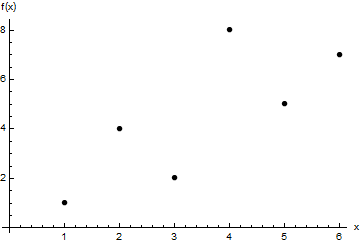
\includegraphics[scale=0.5]{fig/disc-data.png}
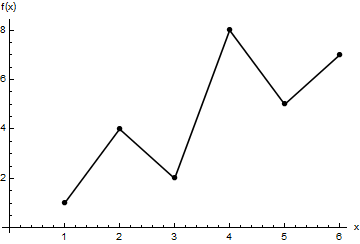
\includegraphics[scale=0.5]{fig/disc-data-line.png}
\caption{硬邦邦的插值}
\label{fig-disc-data}
\end{figure}

但是这样一来每个数据点都是“尖的”,如果要让图像更光滑,可以规定每个数据点两边曲线的斜率必须相同,并且等于它左右两个数据点连线的斜率(最左边和最右边的数据点可以另外规定)。这样一来,数据点上就存在函数的一阶导数。

也就是说,在每两个点之间画一条曲线段,它的两个端点和两端的导数已经确定,共有四个约束条件,如图\ref{fig-cubic-interpo}。三次函数$f(x)=a x^3+b x^2+c x+d$有四个待定系数,所以我们认为这条曲线是三次函数,然后用四个约束条件解出四个待定系数,这就是三次插值。
\begin{figure}[htb]
\centering
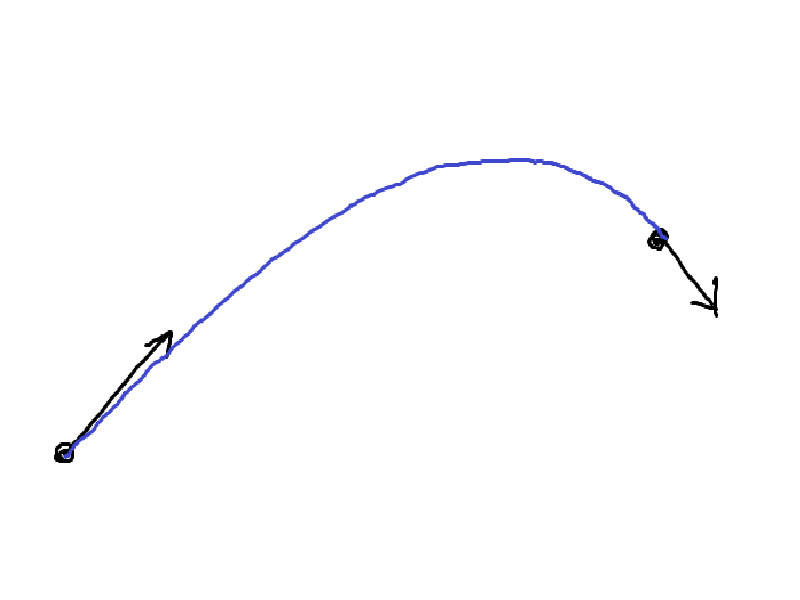
\includegraphics[scale=0.5]{fig/cubic-interpo.png}
\caption{两端的位置和方向确定的曲线段}
\label{fig-cubic-interpo}
\end{figure}

现在来算一下这些系数。简单起见,设曲线段的两端为$(-1,y_1),(1,y_2)$,导数分别为$y'_1,y'_2$。如果两端不在$-1$和$1$,可以平移和缩放$x$轴来实现。解方程组
\begin{equation*}
\begin{cases}
y_1=-a+b-c+d \\
y_2=a+b+c+d \\
y'_1=3 a-2 b+c \\
y'_2=3 a+2 b+c
\end{cases} \Rightarrow \begin{cases}
a=\frac{1}{4}(y_1-y_2+y'_1+y'_2) \\
b=\frac{1}{4}(-y'_1+y'_2) \\
c=\frac{1}{4}(-3 y_1+3 y_2-y'_1-y'_2) \\
d=\frac{1}{4}(2y_1+2y_2+y'_1+y'_2)
\end{cases}
\end{equation*}

上面的数据点用三次插值的结果如图\ref{fig-disc-data-cubic}。PS之类的软件放大图片的时候用的一般是三次插值,虽然最近几年出现了更厉害的方法。如果给定曲线两端的二阶导数甚至更高阶导数,也可以用更高次的多项式实现插值。
\begin{figure}[htb]
\centering
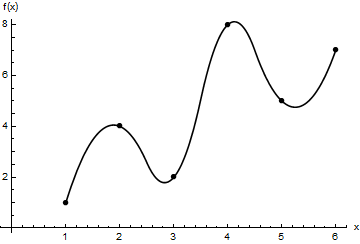
\includegraphics[scale=0.5]{fig/disc-data-cubic.png}
\caption{比较光滑的插值}
\label{fig-disc-data-cubic}
\end{figure}
\section{拉格朗日插值}
三次插值利用相邻的四个数据点来确定曲线段两端的位置和方向,能不能同时考虑所有数据点呢?如果有$n$个数据点,用一个$n-1$次多项式就能经过这些点,称为拉格朗日多项式。

最简单的想法是把$n$个点的坐标代入$n-1$次多项式,解出$n$个待定系数。其实可以直接猜出答案:设数据点为$(x_i,y_i)(i=1,2,\dots,n)$,那么拉格朗日多项式$L(x)=\sum_{i=1}^n y_i l_i(x)$,其中$l_i(x)=\prod \frac{x-x_j}{x_i-x_j}(j=1,2,\dots,n, i \ne j)$。

为什么要这样猜呢?令$x=x_k(1 \le k \le n)$,如果$i=k$,那么$l_i$中相乘的每项都是$1$,否则$l_i$中有一项的分子是$x_k-x_k=0$。也就是说,$l_i(x_k)=\begin{cases} 1, &i=k \\ 0, &i \ne k \end{cases}$,$L(x_k)=y_k$。而且$L(x)$确实是$n-1$次多项式。既然猜出来了,它就是唯一满足条件的多项式。

同样的数据点用拉格朗日插值的结果如图\ref{fig-disc-data-lag}。拉格朗日插值不仅适用于内插,也经常用于外推,图中画出了数据点以外的一段。可以看出,数据点附近的图像会向上和向下超出数据点,比三次插值更加明显。
\begin{figure}[htb]
\centering
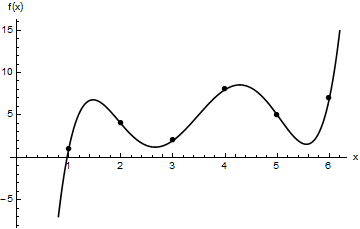
\includegraphics[scale=0.5]{fig/disc-data-lag.png}
\caption{飞起来的插值}
\label{fig-disc-data-lag}
\end{figure}

实际情况下很难说哪种插值更好,有时候需要通过更多实验数据来判断,有时候则有归一化等限制条件。

$n-1$次多项式$L(x)=a_0+a_1 x+a_2 x^2+\dots+a_{n-1} x^{n-1}$可以用$n$个系数$a_i$确定,也可以用$n$个点确定。不管用前面的秦九韶算法还是这里的拉格朗日插值,计算$L(x)$的复杂度都是$O(n^2)$。

如果你熟悉矩阵的求逆,还可以这样理解:把方程组
\begin{align*}
y_1&=L(x_1)=a_0+x_1 a_1+x_1^2 a_2+\dots+x_1^{n-1} a_{n-1} \\
y_2&=L(x_2)=a_0+x_2 a_1+x_2^2 a_2+\dots+x_2^{n-1} a_{n-1} \\
&\dots \\
y_n&=L(x_n)=a_0+x_n a_1+x_n^2 a_2+\dots+x_n^{n-1} a_{n-1}
\end{align*}

看成矩阵方程$\mathbf{y}=\mathbf{V} \mathbf{a}$,其中
\begin{equation*}
\mathbf{V}=\begin{bmatrix}
1 & x_1 & x_1^2 & \dots & x_1^{n-1} \\
1 & x_2 & x_2^2 & \dots & x_2^{n-1} \\
\vdots & \vdots & \vdots & \ddots & & \vdots \\
1 & x_n & x_n^2 & \dots & x_n^{n-1}
\end{bmatrix}
\end{equation*}

称为\emph{范德蒙矩阵},拉格朗日插值就是对$\mathbf{V}$求逆。

(小学生找规律的题目可以用拉格朗日插值来解决。比如$12,14,16,32,(\pheq),36$,可以算出$a_n=-\frac{21}{20} n^4+\frac{77}{6} n^3-\frac{203}{4} n^2+\frac{481}{6} n-\frac{146}{5}$,空格应该填$a_5=\frac{254}{5}$。小朋友们,你们说对不对呀?)
\section{求函数的零点;牛顿法;快速开平方和除法}
现在的科研中很多计算都要用电脑来完成。电脑并不擅长对方程进行移项、因式分解之类的运算,算出一个含有字母的式子,也就是解析解(虽然有软件专门做这些事情);而擅长通过大量加法和乘法之类的简单运算,算出一个很多位小数的近似值,也就是数值解。传说中的\emph{哥德尔定理}告诉我们,数学当中总有一些方程是求不出解析解的。即使能求出,也需要大量的计算,这时候数值解更加实用。

解方程$f_1(x)=f_2(x)$很容易转化为求函数$f(x)=f_1(x)-f_2(x)$的零点$x_0$,所以我们只讲后者。函数的极值也可以转化为它的导数的零点。

如果误差范围是$\Delta x$,而我们知道零点在区间$(x_1,x_2)$内,最简单的想法就是试根:把区间每隔$\Delta x$分成一段,算出每个分割点的函数值,如果相邻两个点的函数值符号不同,零点就在中间。这种方法的复杂度为$O(\frac{l}{\Delta x}),l=x_2-x_1$。

如果知道$f(x)$在区间上单调,还可以用二分法,复杂度为$O(\log \frac{l}{\Delta x})$($\log$的底数是$2$,$10$还是$\rme$之类的无所谓,相当于$O$里面乘一个常数),明显比直接试根要快。

如果利用导数$f'(x)$,还有更快的方法。我们猜:$|f'(x)|$越小,$x$就越靠近$x_0$,如图\ref{fig-newton-iter}。
\begin{figure}[htb]
\centering
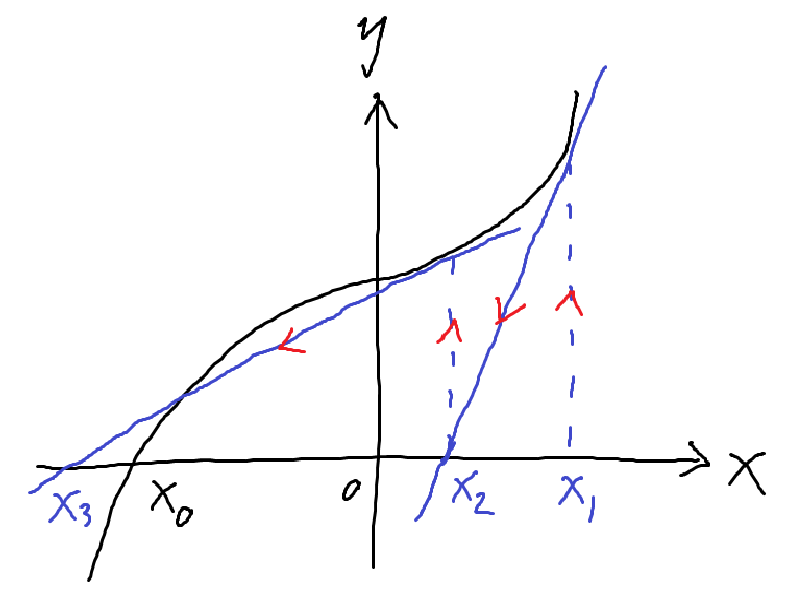
\includegraphics[scale=0.5]{fig/newton-iter.png}
\caption{许多情况下这样猜是有道理的}
\label{fig-newton-iter}
\end{figure}

先在函数图象上随便选一个初始位置$(x_1,f(x_1))$。过$(x_n,f(x_n))$的切线为$y=f'(x_n)(x-x_n)+f(x_n)$,令$x_{n+1}=x_n-\frac{f(x_n)}{f'(x_n)}$,也就是切线与$x$轴的交点。不断重复(或者说迭代),直到满足误差范围。这就是求函数零点的牛顿法。(你可以想一想$f(x)$正负和$f'(x)$正负这四种情况下,$x_n$的变化情况)

这个方法有多快呢?不妨设$x_0=0$,把$f(x)$展开成级数$a_1 x+a_2 x^2+\dots$,每次迭代之后,$a_1 x$这一项就消掉了,剩下二次及以上的项。(当然$a_2$也会有变化,你可以自己算一下)也就是说,每迭代一次,误差大约平方一次,有效位数增加一倍。

如果初始误差是$l(l \ll 1)$,迭代$n$次后误差就是$l^{2^n}$,最终$l^{2^n}<\Delta x$,所以复杂度是$O(\log \log \frac{l}{\Delta x})$,有些地方说它是\emph{二阶收敛}的。

现在来看牛顿法的一些应用。比如计算$\sqrt{A}$,可以构造函数$f(x)=x^2-A$($f(x)$中当然不能出现$\sqrt{A}$),用牛顿法得到$x_{n+1}=\frac{1}{2}(x_n+\frac{A}{x_n})$,这就是多年前初中要学的手算平方根的方法。

再比如计算$\frac{1}{A}$,可以构造函数$f(x)=\frac{1}{x}-A$,用牛顿法得到$x_{n+1}=x_n(2-A x_n)$,这样就用减法和乘法代替了除法。如果精度要求不高,这样比列竖式要快一些。

但是,牛顿法难以判断$f(x)$根本没有零点的情况。即使有零点,牛顿法也不一定收敛,如图\ref{fig-newton-iter-boom}。这跟初始位置的选取有关,需要其他方法来判断合适的初始位置,这里就不仔细讲了。
\begin{figure}[htb]
\centering
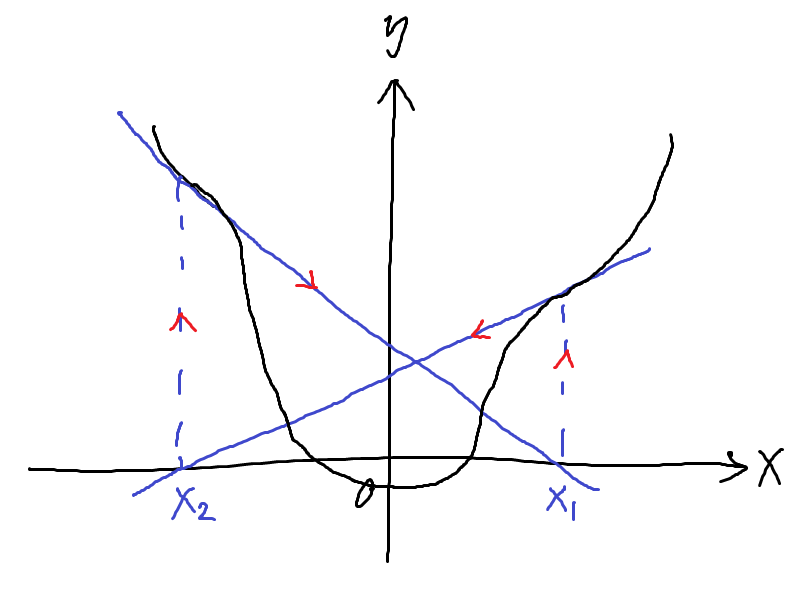
\includegraphics[scale=0.5]{fig/newton-iter-boom.png}
\caption{牛顿气得从棺材里爬了出来}
\label{fig-newton-iter-boom}
\end{figure}
\section{求导}
要计算$f'(x)$的近似值,可以把$f(x)$展开:$f(x+h)=f(x)+f'(x) h+\frac{1}{2} f''(x) h^2+\dots(h \ll 1)$。最简单的想法是$f'(x)=\frac{f(x+h)-f(x)}{h}$,实际情况下$h$不可能无限小,右边的结果为$f'(x)+\frac{1}{2} f''(x) h+\dots$,误差为$O(h)$。$h$减小,展开式的误差会减小,但除以$h$造成的误差会增大。

如果同时利用$f(x-h)=f(x)-f'(x) h+\frac{1}{2} f''(x) h^2+\dots$,可以得到更准确的结果:$f'(x)=\frac{f(x+h)-f(x-h)}{2 h}$,这样结果中的$\frac{1}{2} f''(x) h$就消掉了,误差为$O(h^2)$。卡西欧计算器用的就是这种方法,取$h=0.001$。

还能算出$f''(x)=\frac{f(x+h)-2 f(x)+f(x-h)}{h^2}$,误差为$O(h)$。

取更多的点,结果还能更准确。比如在$x$附近取四个点,可以解方程组
\begin{equation*}
\begin{cases}
f(x-2 h)=f(x)-2 f'(x) h+2 f''(x) h^2-\frac{4}{3} f^{(3)}(x) h^3+\frac{2}{3} f^{(4)}(x) h^4-\dots \\
f(x-h)=f(x)-f'(x) h+\frac{1}{2} f''(x) h^2-\frac{1}{6} f^{(3)}(x) h^3+\frac{1}{24} f^{(4)}(x) h^4-\dots \\
f(x+h)=f(x)+f'(x) h+\frac{1}{2} f''(x) h^2+\frac{1}{6} f^{(3)}(x) h^3+\frac{1}{24} f^{(4)}(x) h^4+\dots \\
f(x+2 h)=f(x)+2 f'(x) h+2 f''(x) h^2+\frac{4}{3} f^{(3)}(x) h^3+\frac{2}{3} f^{(4)}(x) h^4+\dots
\end{cases}
\end{equation*}

这是四元一次方程组,解得$f'(x)=\frac{1}{12 h}(-f(x+2 h)+8 f(x+h)-8 f(x-h)+f(x-2 h))$,误差为$O(h^5)$。还能顺便算出$f''(x),f^{(3)}(x),f^{(4)}(x)$,这里就不写出来了。
\section{积分}
首先,数值方法只能算定积分。这次最简单的想法是
\begin{equation*}
\int_a^b f(x) \opd x=\sum_{n=\frac{a}{h}}^{\frac{b}{h}} f(n h) h
\end{equation*}

它的几何意义就是把曲线下的面积近似成很多矩形的面积,也可以借助差分与求和来理解。令$F(x)=\int f(x) \opd x$,可以把它展开:$F(x+h)-F(x)=f(x) h+\frac{1}{2} f'(x) h^2+\dots$。然后还要换元:$x=n h$。保留$O(h)$的项,两边求和就得到了上面的式子,误差为$\Sigma O(n^2)$。

如果保留$O(h^2)$的项,可以得到更准确的结果:
\begin{equation*}
\int_a^b f(x) \opd x=\sum_{n=\frac{a}{h}}^{\frac{b}{h}} f(n h) h+\frac{1}{2} f'(n h) h^2
\end{equation*}

这里需要计算$f'(x)$的准确值,但是也可以用刚才的近似值$f'(x)=\frac{f(x+h)-f(x)}{h}$代替,得到
\begin{equation*}
\int_a^b f(x) \opd x=\sum_{n=\frac{a}{h}}^{\frac{b}{h}} \frac{1}{2} (f((n+1) h)+f(n h)) h
\end{equation*}

它的几何意义则是用直角梯形代替矩形,也就是把曲线近似成折线段,误差为$\Sigma O(n^3)$。如果把曲线近似成抛物线段,结果还能更准确,但是推导起来比较麻烦,这里也不仔细讲了。
\begin{figure}[htb]
\centering
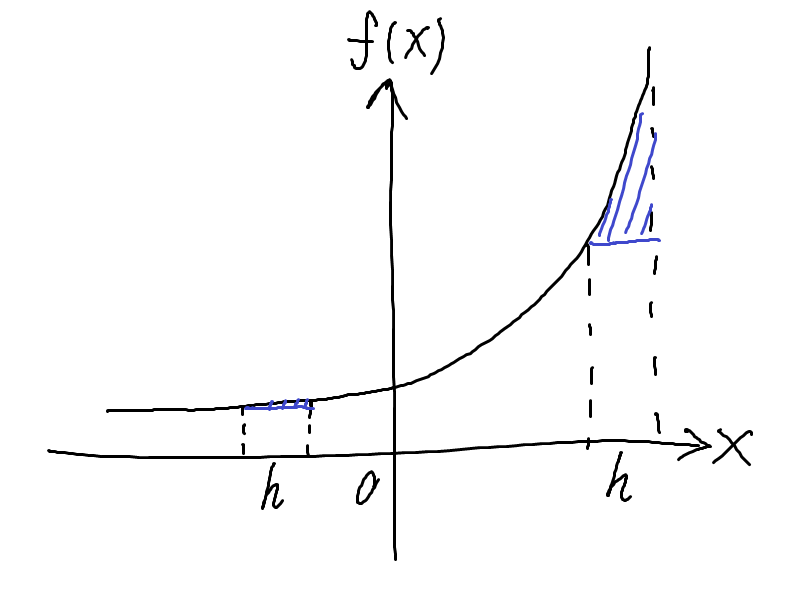
\includegraphics[scale=0.5]{fig/adjust-h.png}
\caption{把曲线下的面积近似成矩形}
\label{fig-adjust-h}
\end{figure}

到目前为止$h$在整个计算过程中是固定的。如图\ref{fig-adjust-h},简单起见,把曲线下的面积向下近似成矩形,蓝色部分是产生的误差。可以看出,$|f'(x)|$越大,误差就越大,这时我们可以减小对应的矩形的宽度,比如
\begin{equation*}
\int_a^b f(x) \opd x=\sum_{\{x_i\}} f(x_i) \frac{h}{1+f'(x_i)}
\end{equation*}

$f'(x_i)$前面留一个$1$是为了防止$f'(x_i)$很小的时候爆掉。这里求和的范围比较难写,反正就是把区间$(a,b)$分成一个个长为$\frac{h}{1+f'(x_i)}$的部分,每个部分里随便取一个$x_i$(诶这是循环定义吗)。真的用电脑算的时候还有许多细节问题。

许多微分方程可以转化为积分,然后用这些方法求出数值解。如果$f(x)$是复变函数,以后我们会更深入地学习它的导数与积分的联系。
\section{蒙特卡罗方法}
这个方法的名字好像很厉害,其实就是利用随机数来解决问题。

比如我们要算圆的面积,量纲分析可以得到$S=A r^2$,然后要确定系数$A$。我们知道判断一个点在圆内的方法是$x^2+y^2<r^2$,但是假装不知道怎么从它推导出圆的面积公式。现在画一个边长为$2$的正方形,我们知道它的面积为$4$,内接圆的半径$r=1$。用电脑在正方形里随机选取$10000$个点(或者说生成$10000$个随机数对$(x,y),-1<x<1,-1<y<1$),如图\ref{fig-monte-carlo-circle}。然后数一数,共有$7879$个点在圆内,所以$S=\frac{4 \times 7879}{10000}=3.1516$,我们可以猜$A=\pi$。
\begin{figure}[htb]
\centering
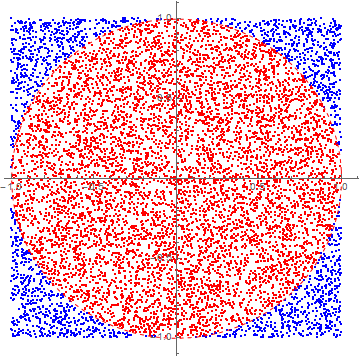
\includegraphics[scale=0.5]{fig/monte-carlo-circle.png}
\caption{对密集恐惧症患者造成伤害}
\label{fig-monte-carlo-circle}
\end{figure}

10000个点对电脑来说不算多,可以在几毫秒内完成。如果增加点的数量,结果会更准确。

当然这是个很简单的例子,用面积元积分也可以算出准确值。如果要算$n$维球体的体积,判断依据和刚才差不多:$\sum_{i=1}^n x_i^2<r^2$。随着$n$的增加,用体积元积分会十分复杂,而蒙特卡罗方法的步骤是差不多的。

(但是!随着维度增加,球体和立方体的体积比值会迅速减小,如果用蒙特卡罗方法,到后面很少有点会落在球体内。事实上还有高斯积分之类奇怪的方法可以推导$n$维球体的体积公式)

还有一个问题:我们随机取了很多点,如果在$x-y$坐标系中画小方格来取点不是更方便吗?(而且计算机生成小方格比随机数快多了)这其实是一个采样的过程。算圆的面积确实可以画小方格来采样,但是许多问题是画不出这样的“小方格”的。

比如这样一个问题:在一维情况下,把$N$只兔子放在一个长为$L$的笼子里,如图\ref{fig-rabbit-box}。每只兔子看作长为$a$的线段,兔子不能相互重叠,也不能与两边的墙重叠。现在求坐标为$x$的点被兔子占据的概率。
\begin{figure}[htb]
\centering
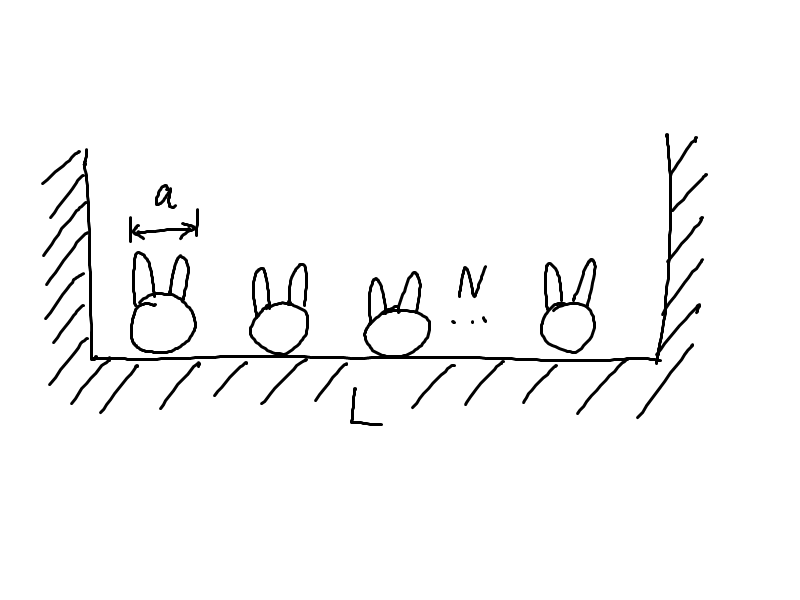
\includegraphics[scale=0.5]{fig/rabbit-box.png}
\caption{向蔡老师致敬}
\label{fig-rabbit-box}
\end{figure}

你觉得还能画出小方格吗?一种想法是以每只兔子的坐标$x_i$为坐标轴,建立$N$维坐标系(也就是兔子的\emph{位形空间}),在里面画小方格。但是随着$N$的增加和小方格边长的减小(精度的提高),小方格的数量会迅速(指数级)增加,超出电脑的计算能力。这时候需要更加巧妙的采样方法,这里就不仔细讲了。

(其实这个问题在统计力学中非常重要,与\emph{熵力}有关,也是我个人感兴趣的问题,以后应该会专门讲)

在用电脑计算的过程中,我们需要确保产生的是随机数。如果产生的数容易分布在某一块区域里,结果就不准了。事实上,不管是用程序产生随机数,还是验证一个程序产生的确实是随机数,都是不容易的问题。但是我们可以相信,现在的编程语言提供的随机数功能够用了。

要验证产生的是随机数,一个容易想到的标准是:产生区间$(a,b)$内的随机数,一次产生$N$个,然后在$(a,b)$中任意取一个长度为$l$的区间,要求其中的随机数个数$n$与$N$和$l$都成正比。这样的“随机数”称为\emph{低差异序列}。
\vfill
\begin{figure}[htb]
\centering
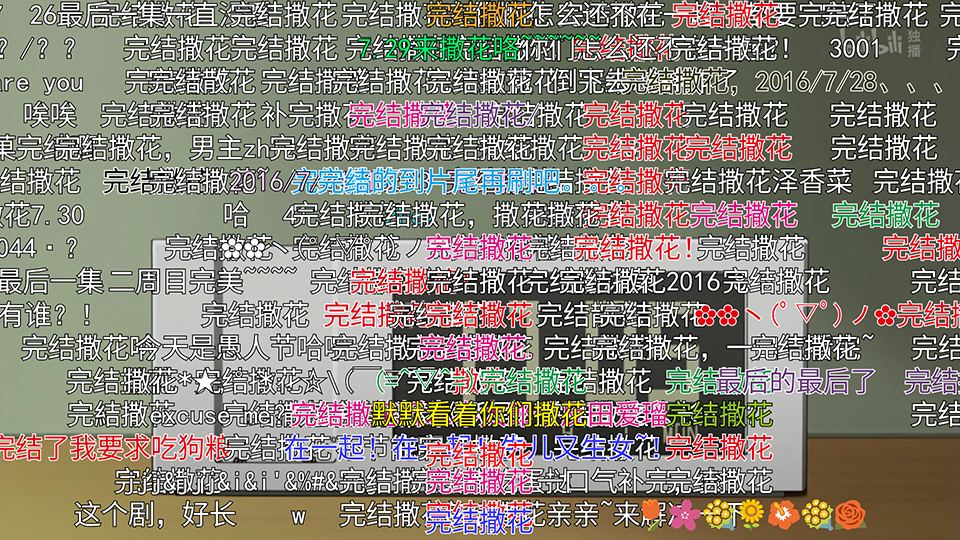
\includegraphics[width=\textwidth]{fig/final-flower.png}
\caption{完结撒花}
\label{fig-final-flower}
\end{figure}
\vfill
